\section{16. März 2012}

\question{Diskutieren der unterschiedlichen Überlegungen in der Valenzbindugsnäherung (VB) und in der Molekularorbitalnäherung (MO) zur Beschreibung der Molekülbindung in einem 2-atomigen Molekül}
\label{q:41}
\textbf{VB-Näherung}
\begin{itemize}
   
    \item erklärt Paarung von Elektronen durch Überlappung von Orbitale und Pi- und Sigma-Bindungen
    \item erklärt Hybridorbitale, aber liefert KEINE Details über Molekülorbitale
    \item im Grundzustand können zwei Elektronen mit $\uparrow \downarrow$ Spins untergebracht werden
    \item zwei lokalisierte Elektronen um Kerne A und B
    \item beide Elektronen werden betrachtet, sodass für beide Wahrscheinlichkeitsamplituden $\Psi_1$ und $\Psi_2$ ein Produktansatz der Atomorbitale notwendig ist 
    \item Besetzung des Molekülorbitals wird mit Linearkombination von $\Psi_1$ und $\Psi_2$ durch Pauli-Prinzip erzwungen
\end{itemize}


\noindent
\textbf{MO-Näherung}
\begin{itemize}
    \item basiert auf bindenden und antibindenden Molekülorbitalen
    \item erklärt nicht die Hybridisierung des Orbitale
    \item ein Elektron betrachtet, dass sich in $\Phi_A$ als auch in $\Phi_B$ aufhalten kann, sodass für dieses Molekülorbital-Ansatz notwendig ist (wobei $\Phi_A$ und $\Phi_B$ atomare Wellenfunktionen)
    \item für Besetzung des Molekülorbitals mit zwei Elektronen wird Produktansatz verwendet
\end{itemize}
\question{Skizzieren der bindenden und antibindenden Wellenfunktionen in einem homonuklearen 2-atomigen Molekül}
\label{q:42}
\begin{figure}[H]
    \centering
   \begin{minipage}[b]{.4\linewidth} % [b] => Ausrichtung an \caption
      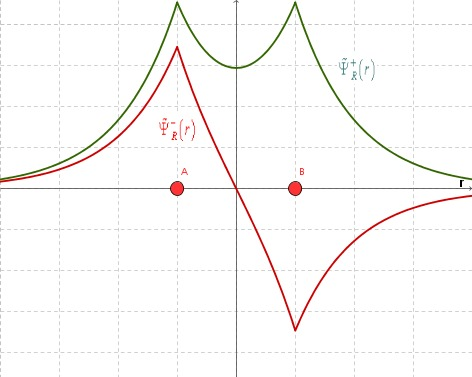
\includegraphics[width=\linewidth]{resources/16-03-2012/sym_und_antisymm_Wellenfunktion.jpeg}
      \caption{\textbf{Wellenfunktionen} symmetrische (bindend, grün) und antisymmetrische (antibindende, rot) Wellenfunktion}
   \end{minipage}
   \hspace{.1\linewidth}% Abstand zwischen Bilder
   \begin{minipage}[b]{.4\linewidth} % [b] => Ausrichtung an \caption
      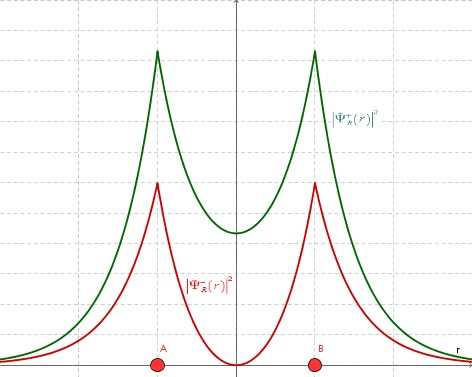
\includegraphics[width=\linewidth]{resources/16-03-2012/Wahrscheinlichkeitsdichten.jpeg}
      \caption{Wahrscheinlichkeitsdichten der symmetrischen (bindend, grün) und antisymmetrischen (antibindende, rot) Wellenfunktion}
   \end{minipage}
\end{figure}
\question{Diskutieren des Schwigungs-Rotations Spektrums eines 2-atomigen Moleküls}
\label{q:43}
\begin{itemize}
    \item Spektren zweiatomiger Moleküle entstehen durch Rotations- und Schwingungsübergänge
    \item im realen Molekül führen Kerne um Gleichgewichtsabstand $R_e$ Schwingungen aus, sodass sich Kernabstand $R$ während Rotation des Moleküls ändert
    \item \textbf{Rotationsspektren}
        \begin{itemize}
            \item entstehen durch Absorption des Moleküls im Ultrarot-Bereich
            \item durch Energieaufnahme kommt es zu Strahlungsübergänge zwischen den Rotationszuständen
            \item in einfachster Näherung wird Molekül als \textbf{starrer Rotator} betrachtet, der sich mit konstantem Kernabstand $R=R_e$=const um Schwerpunktachse dreht. Rotationsenergie $E_{rot}$ ,als Termwert $F_{rot}$, hat bei $R=R_e$ diskrete Werte, siehe \ref{RotEnergie_starr} \ref{Termwert_RotE}. Die Abstände der Energieniveaus $\Delta E_{rot}$ nehmen linear zu, siehe \ref{Abstaende_Eniveaus_starr}.

                \begin{equation}
                E_{rot} = \frac{J(J+1)\hbar^2}{2MR_e^2}
                \label{RotEnergie_starr}
                \end{equation}

                \begin{equation}
                F_{rot}(J)=B_eJ(J+1)=\frac{\hbar}{4\pi cMR_e^2}J(J+1)
                \label{Termwert_RotE}
                \end{equation}

                \begin{equation}
                \Delta E_{rot}=E_{rot}(J+1)-E_{rot}=\frac{(J+1)\hbar^2}{I}
                \label{Abstaende_Eniveaus_starr}
                \end{equation}

            \item beim \textbf{nicht starren Rotator} (Zentrifugalkraft berücksichtigt) besteht elastische Bindung zwischen Atomen mit Federkonstante k. Der Kernabstand vergößert sich von $R_e$ auf $R$, dabei wird Trägheitsmoment $I$ kleiner und Rotationsenergie $F_{rot}$ größer, siehe \ref{RotE_nichtstarr}. Die Spektrallinienwachsen rücken mit steigender Rotationsquantenzahl J=0,1,2,... näher zusammen.

                \begin{equation}
                   F_{rot}=B_eJ(J+1)-D_eJ^2(J+1)^2+...
                   \label{RotE_nichtstarr}
                    \end{equation}
    \begin{figure}[H]
    \centering
   \begin{minipage}[b]{.3\linewidth}
      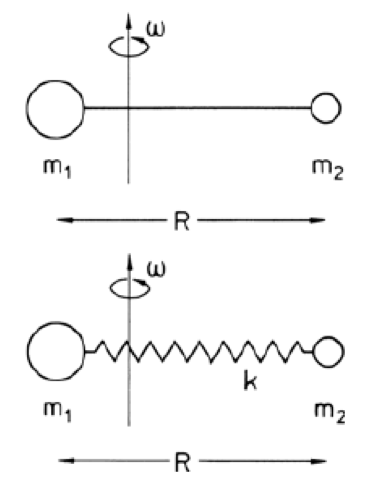
\includegraphics[width=\linewidth]{resources/16-03-2012/StarrervsnichtstarrerRotor.png}
      \caption{starrer Rotor vs nicht starrer Rotor}
   \end{minipage}
   \hspace{.1\linewidth}
   \begin{minipage}[b]{.3\linewidth} 
      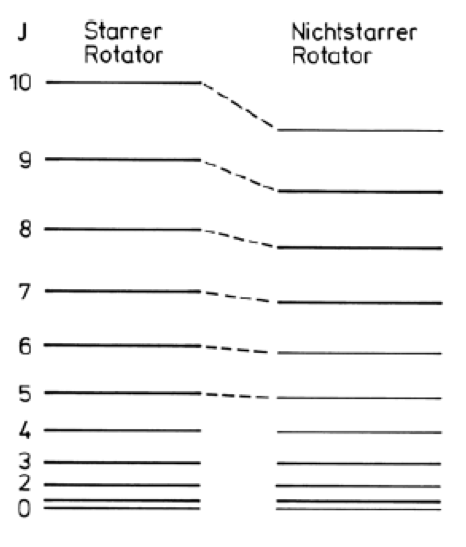
\includegraphics[width=\linewidth]{resources/16-03-2012/2starrervsnichtstarrerrotos.png}
      \caption{Übergänge starrer vs nicht starrer Rotor}
   \end{minipage}
    \end{figure}
                
        \end{itemize}

    \item \textbf{Rotationsschwingungsspektren}
        \begin{itemize}
            \item entstehen durch Absorption/Emission des Moleküls im Infrarot-Bereich, wobei Rotation und Schwingung gleichzeitig verändert werden
            \item jede Bande des Rotationsschwingungsspektrums entspricht einem Schwingungsübergang
            \item in einfachster Näherung bilden schwingende Atome des Moleküls einen \textbf{harmonischen Oszillator} mit diskreten Energie $E_{vib}$, siehe \ref{EVib_harmonisch}, und gleich große Energieabstände $\Delta E_{vib}$, siehe \ref{EVib_Abstaende}. Potential kann durch Parabelpotential angenähert werden.

                \begin{equation}
                    E_{vib}(\nu)=(\nu+\frac{1}{2})\hbar \omega
                \label{EVib_harmonisch}
                \end{equation}

                \begin{equation}
                \Delta E_{vib}=\hbar \omega
                \label{EVib_Abstaende}
                \end{equation}

            \item bei Näherung als \textbf{anharmonischer Oszillator} rücken die Enrgieniveaus mit zunehmender Schwingungsquantenzahl $\nu$=0,1,2,... näher zusammen und konvergieren gegen Dissoziationsenergie des Moleküls. Potential kann durch Morse-Potential angenähert werden.
        \end{itemize}

\end{itemize}


\begin{figure}[H]
    \centering
   \begin{minipage}[b]{.4\linewidth}
      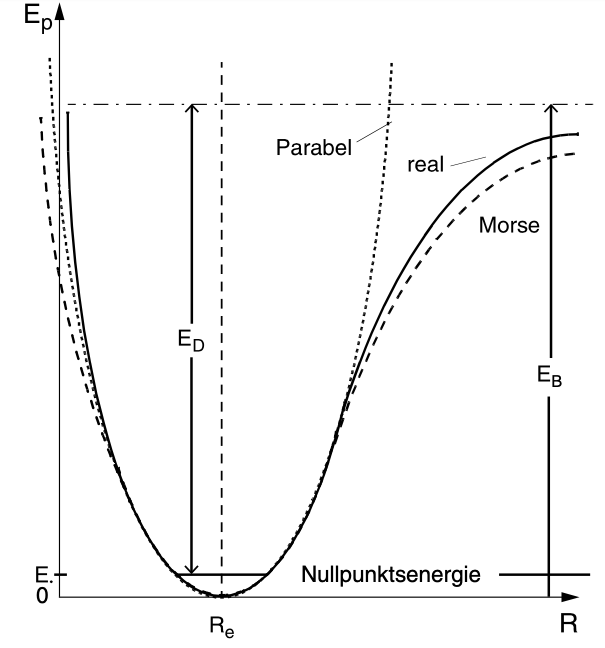
\includegraphics[width=\linewidth]{resources/16-03-2012/Vergleich_ParabelMorseReal.png}
      \caption{Vergleich zwischen Parabel-, Morse- und realen Potentials}
   \end{minipage}
   \hspace{.1\linewidth}
   \begin{minipage}[b]{.4\linewidth} 
      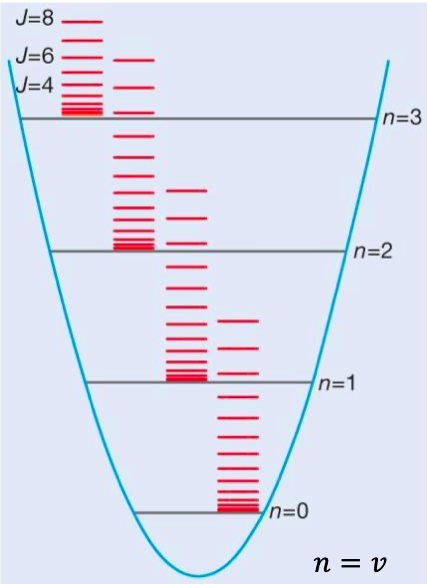
\includegraphics[width=0.8\linewidth]{resources/16-03-2012/SchwingugsRotatioinsspektrum.png}
      \caption{Darstellung der Rotations- und Schwingungsniveaus, jedem Schwingungsniveau ist Reihe von Rotationsniveaus zugeordnet}
   \end{minipage}
    \end{figure}
\question{Diskutiere die chemische Bindung im Li2 Molekül}
\label{q:44}
Jedes Lithium-Atom liefert jeweils 3 Elektronen, insgesamt also 6 Elektronen. 
Somit sind die Molekülorbitale ($1\sigma_g)^2$ ($1\sigma_u)^2$ ($2\sigma_g)^2$ besetzt. 
Da das ($2\sigma_g)$ Orbital besetzt ist, handelt es sich um eine stabile Bindung. 
Es gibt ein bindendes Elektronenpaar und daher handelt es sich um eine kovalente Bindung.

\question{Was versteht man unter dem Franck-Condon-Prinzip? Diskutiere die Intensität von Schwingungsbänden in einem Molekülspektrum bei einem elektronischen Übergang anhand des Franck-Condon-Prinzips.}
\label{q:45}

\question{Wodurch unterscheidet sich ein fcc Gitter von einem hcp?}
\label{q:46}

fcc- face centered cubic, hcp - hexagonal close packed

\begin{enumerate}
    \item Anordnung der Atome: Im fcc-Gitter sind die Atome auf den Eckpunkten eines Würfels sowie in den Zentren der sechs Flächen platziert. Im hcp-Gitter sind die Atome hexagonal angeordnet.
    \item Einheitszelle: Im fcc-Gitter ist die Einheitszelle ein Würfel, jeder Eckpunkt enthält ein Atom. Im hcp-Gitter ein hexagonales Prisma, jede Basiseben enthält ein Atom.
    \item Schichstruktur: Im fcc-Gitter gibt es keine klaren Schichten, da die Atome gleichmäßig im Raum verteilt sind. Im hcp-Gitter sind die Schichten klar definiert.
    \item Komprimierung: Im fcc-Gitter beträgt a:c : $\sqrt{2}:1$. Im hcp-Gitter beträgt a:c : $\sqrt{3}:2$.
\end{enumerate}

\question{Erläutere den Atomfaktor und den Strukturfaktor bei der Röntgenbeugung.}
\label{q:47}

\question{Skizziere die 1. Brillouin-Zone eines ebenen Parallelogrammgitters.}
\label{q:48}

Zur Erklärung der Konstruktion siehe \autoref{q:28}.
\begin{figure}[H]
    \centering
    \begin{samepage}
        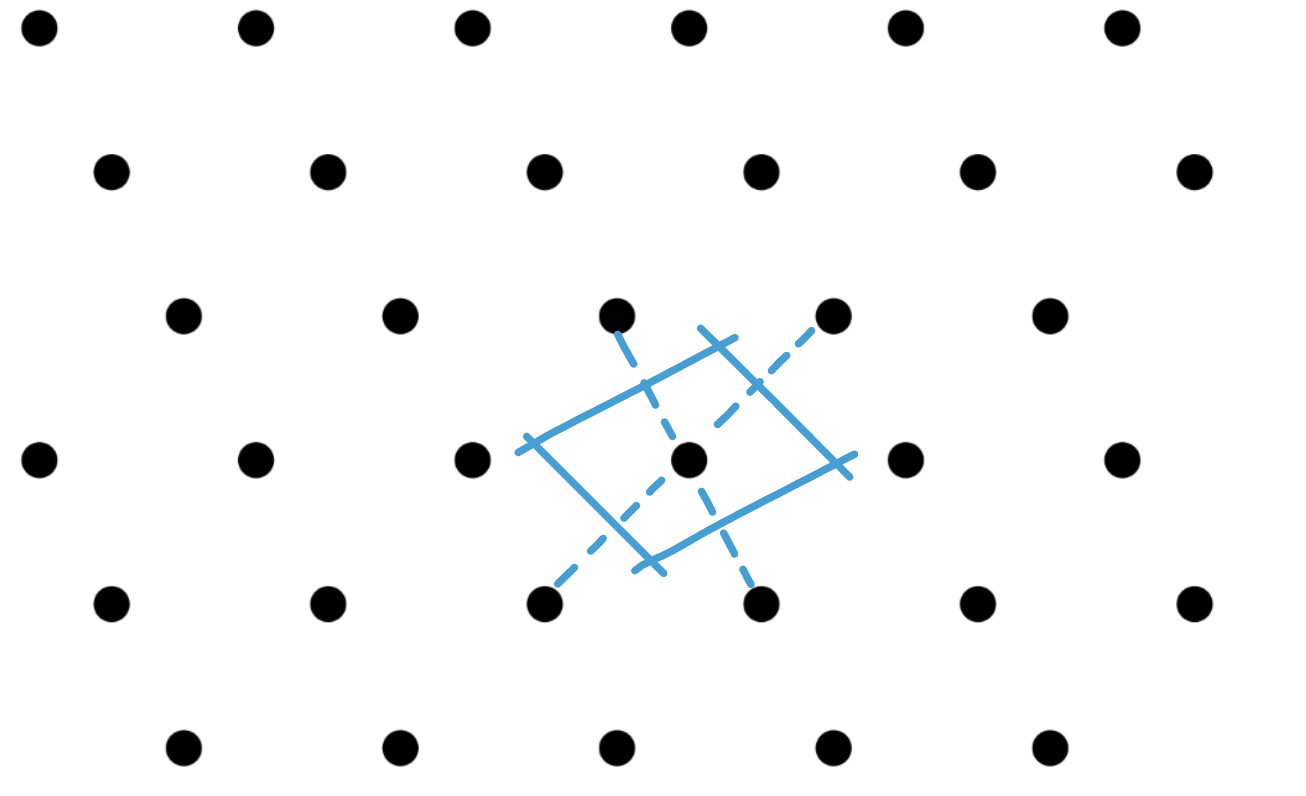
\includegraphics[width=0.4\linewidth]{resources/16-03-2012/BZ1.png}
        \caption[BZ1 Parallelogrammgitter]{1. Brillouin-Zone eines ebenen Parallelogrammgitters}
        \label{fig:BZ1_Parallelogrammgitter}
    \end{samepage}
\end{figure}

\question{Wodurch unterscheidet sich die Dispersionsrelation der Phononen eines primitiven kubischen Gitters von jener eines CsCl-Gitters.}
\label{q:49}

\question{Vergleiche die Einstein- und Debye-Modelle der spez. Wärme. Welche Annahme ist im Einstein Modell zu einfach?}
\label{q:50}

siehe \aqref{40}

\newpage